%\documentclass[12pt,a4paper]{book}\usepackage[utf8]{inputenc}\usepackage[T1]{fontenc}\usepackage{lmodern}\usepackage{hyperref}\usepackage{graphicx}\usepackage[english, frenchb]{babel}\usepackage{listings}	\lstdefinestyle{customstyle}{basicstyle=\footnotesize,breakatwhitespace=false,breaklines=true,captionpos=b,keepspaces=true,tabsize=4,frame=single}\lstset{style=customstyle}\usepackage{menukeys}\begin{document}
\chapter{Basic setup}

\section{Change language}
There are no default languages selected in ArchLinux but the keyboard map is set to 
qwerty\footnote{Most common layout for keyboards} at the beginning. To choose 
your language you have to complete two steps and then the system will be able to 
use it for characters encoding and some softwares as \texttt{nano}.

\subsection{Enable yours}
Before choosing yours it is necessary to enable it in \texttt{/etc/locale.gen}
file with \texttt{locale} tools. 

You will need to use \texttt{nano} to edit the configuration file -- \keys{\ctrl 
+ W} can help you to search -- and remove \og\#\fg{} before the language you want 
to enable (fr\_FR.UTF-8 for example), to save your changes press \keys{\ctrl + X}.
\\
\begin{lstlisting}[language=bash,caption=Enable your language]
$ locale # Current language settings

# Edit the /etc/locale.gen file
$ nano /etc/locale.gen

$ locale-gen # Update available languages
$ locale -a  # See available languages
\end{lstlisting}

\subsection{Change your settings}
The second step is to set the language and configure your keyboard map. 
Notice that you will have to logout for the system to take into account 
changes you made with language setup.
\\ 
\begin{lstlisting}[language=bash,caption=Change language settings]
$ localectl status
  System Locale: n/a  # System language
      VC Keymap: n/a  # Virtual console
     X11 Layout: n/a  # Graphic interface
     
# Change system language (enabled one)
$ localectl set-locale LANG=fr_FR.UTF-8

# List of keymaps, choose the one you want "fr-pc" for example
$ localectl list-keymaps

# Change settings 
# no-convert not update VC with X11 and vice versa
$ localectl set-keymap --no-convert fr-pc     # VC Keymap
$ localectl set-x11-keymap --no-convert fr-pc # X11 Layout

# Logout to apply changes
$ exit
\end{lstlisting}

\section{Configure wifi connexion}
\subsection{Check your dongle}
The first thing you can do is check if your dongle has been recognized by 
the system and can be used.

\begin{lstlisting}[language=bash,caption=Check wifi device]
$ ifconfig -a wlan # All wireless interfaces (also disabled)

# If you see a line with "wlan0" try to enable it
$ ip link set wlan0 up

# If you see again "wlan0" your dongle is working
# Disable it after the check
$ ifconfig wlan # Without -a show only enabled interfaces
$ ip link set wlan0 down
\end{lstlisting}

There are a lot of ways to connect your RPi to a network using a wifi dongle 
but all of them requires to install a package before -- wifi-menu needs 
dialog, iw and wpa\_supplicant are not installed -- so it is necessary to 
use an ethernet wire to begin.

\begin{lstlisting}[language=bash,caption=Install wireless dependencies]
# pacman is the package manager in ArchLinux
#        -S install a new package 
#
# dialog to get wifi-menu interface
# wpa_supplicant for wireless network protected with wpa keys
#
$ pacman -S dialog wpa_supplicant
\end{lstlisting}

\subsection{Searching the internet}
Once you installed all the packages -- synonym for software -- that wifi-menu 
needed to run you can launch it with \og{}\texttt{wifi-menu}\fg{} command.

\begin{figure}[h]
	\centering
	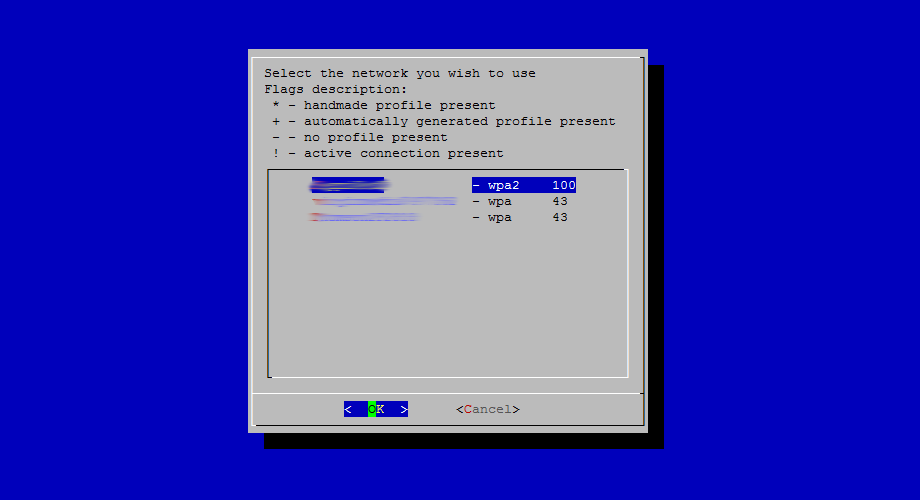
\includegraphics[scale=0.3]{images/WifiMenu.png}
	\caption{wifi-menu interface}
	\label{figure:WifiMenu}
\end{figure}

Then, select your network -- with \keys{\arrowkeyup} and \keys{\arrowkeydown} -- 
, type your password (if required) and you will be connected to your wireless 
network.
\newpage
\section{Create yourself}
\subsection{Simple user}
The default username and password for ArchLinux are \texttt{root/root}, this 
user got all right on the system it means he can do anything -- even break 
the system -- so it is not recommanded to use it.
\\
\begin{lstlisting}[language=bash,caption=Create a new user called jeremy]
$ useradd -m jeremy # Creates user jeremy and his home folder
$ passwd jeremy     # Changes jeremy password
\end{lstlisting}

Now we have a new user account for everydays usage. You can see all users on 
your system with \og{}\texttt{cat /etc/passwd}\fg{} which will display the 
content of the config file for users.

\subsection{Very important user}
It is possible to specify user rights with \texttt{visudo} command, the general syntax for one user is 
the following \og{}\texttt{username machine=(targetuser) commands}\fg{}, 
let's look at some details:


%# Attribute rights with a specific format
%$ visudo
%# Add new line: "jeremy ALL=(ALL) ALL"

\begin{description}
\item[username] name you gave to \texttt{useradd} command
\item[machine] machine on where rights are applied, ALL in general
\item[target user] user that we takes the rights
\item[command] allowed commands separated with one coma -- no spaces --, 
use exclamation mark for banned commands
\end{description}

%\end{document}
